\subsection{Sensitive analysis of the SI-method for the test data}
\label{se:accuracy_SI_method}
Since the significant discrepancy of roll damping between the model test results and the SI-method might be caused by the errors from different components and ship parameters, an sensitive study is carried out to investigate 1) which ship parameters in describing the roll damping contribute most to the discrepancy, and 2) which roll damping components are easily affected by the ship parameters. A so-called ``reference ship" with ship parameters located in the middle of the SI-method applicable boundaries as in Eq. (\ref{eq:SI_limits}) is also used for the investigation. For the sensitive study, only the relatively important ship parameters, i.e., $C_b$,$\frac{Beam}{T}$, $\frac{\overline{OG}}{T}$, $A_0$, $\frac{BK_B}{Beam}$, $\frac{BK_L}{L_{pp}}$, are chosen to investigate the effects of their variation on different roll damping components. 

The results of the sensitive analysis are presented in Fig. \ref{fig:SI_sensitivity}. It can be seen that the wave damping component $B_W$ increases a lot with the absolute value of $\overline{OG}/T$. It can be also seen that the wave damping has an enormous increase when the beam to draught ratio exceeds the input boundary, which seems to be the case for at least one third of the roll decay tests. It can also be noted that most of the ships in the database have midsection coefficients $A_0$ and bilge keel heights outside the limits. The unrealistic prediction of wave damping component $B_W$ in terms of $\frac{Beam}{T}$ and $\frac{\overline{OG}}{T}$ should be further examined. The big variation might be caused by the improper ship parameter $\frac{Beam}{T}$ that is outside the boundaries used in the SI-method. It might be also caused by the semi-empirical separation of different damping components, especially the wave component. In the following, the original Ikeda's method based on strip theory based numerical analysis is used to verify the semi-empirical methods for the estimation of roll damping.  


\begin{figure}[H]
    \centering
    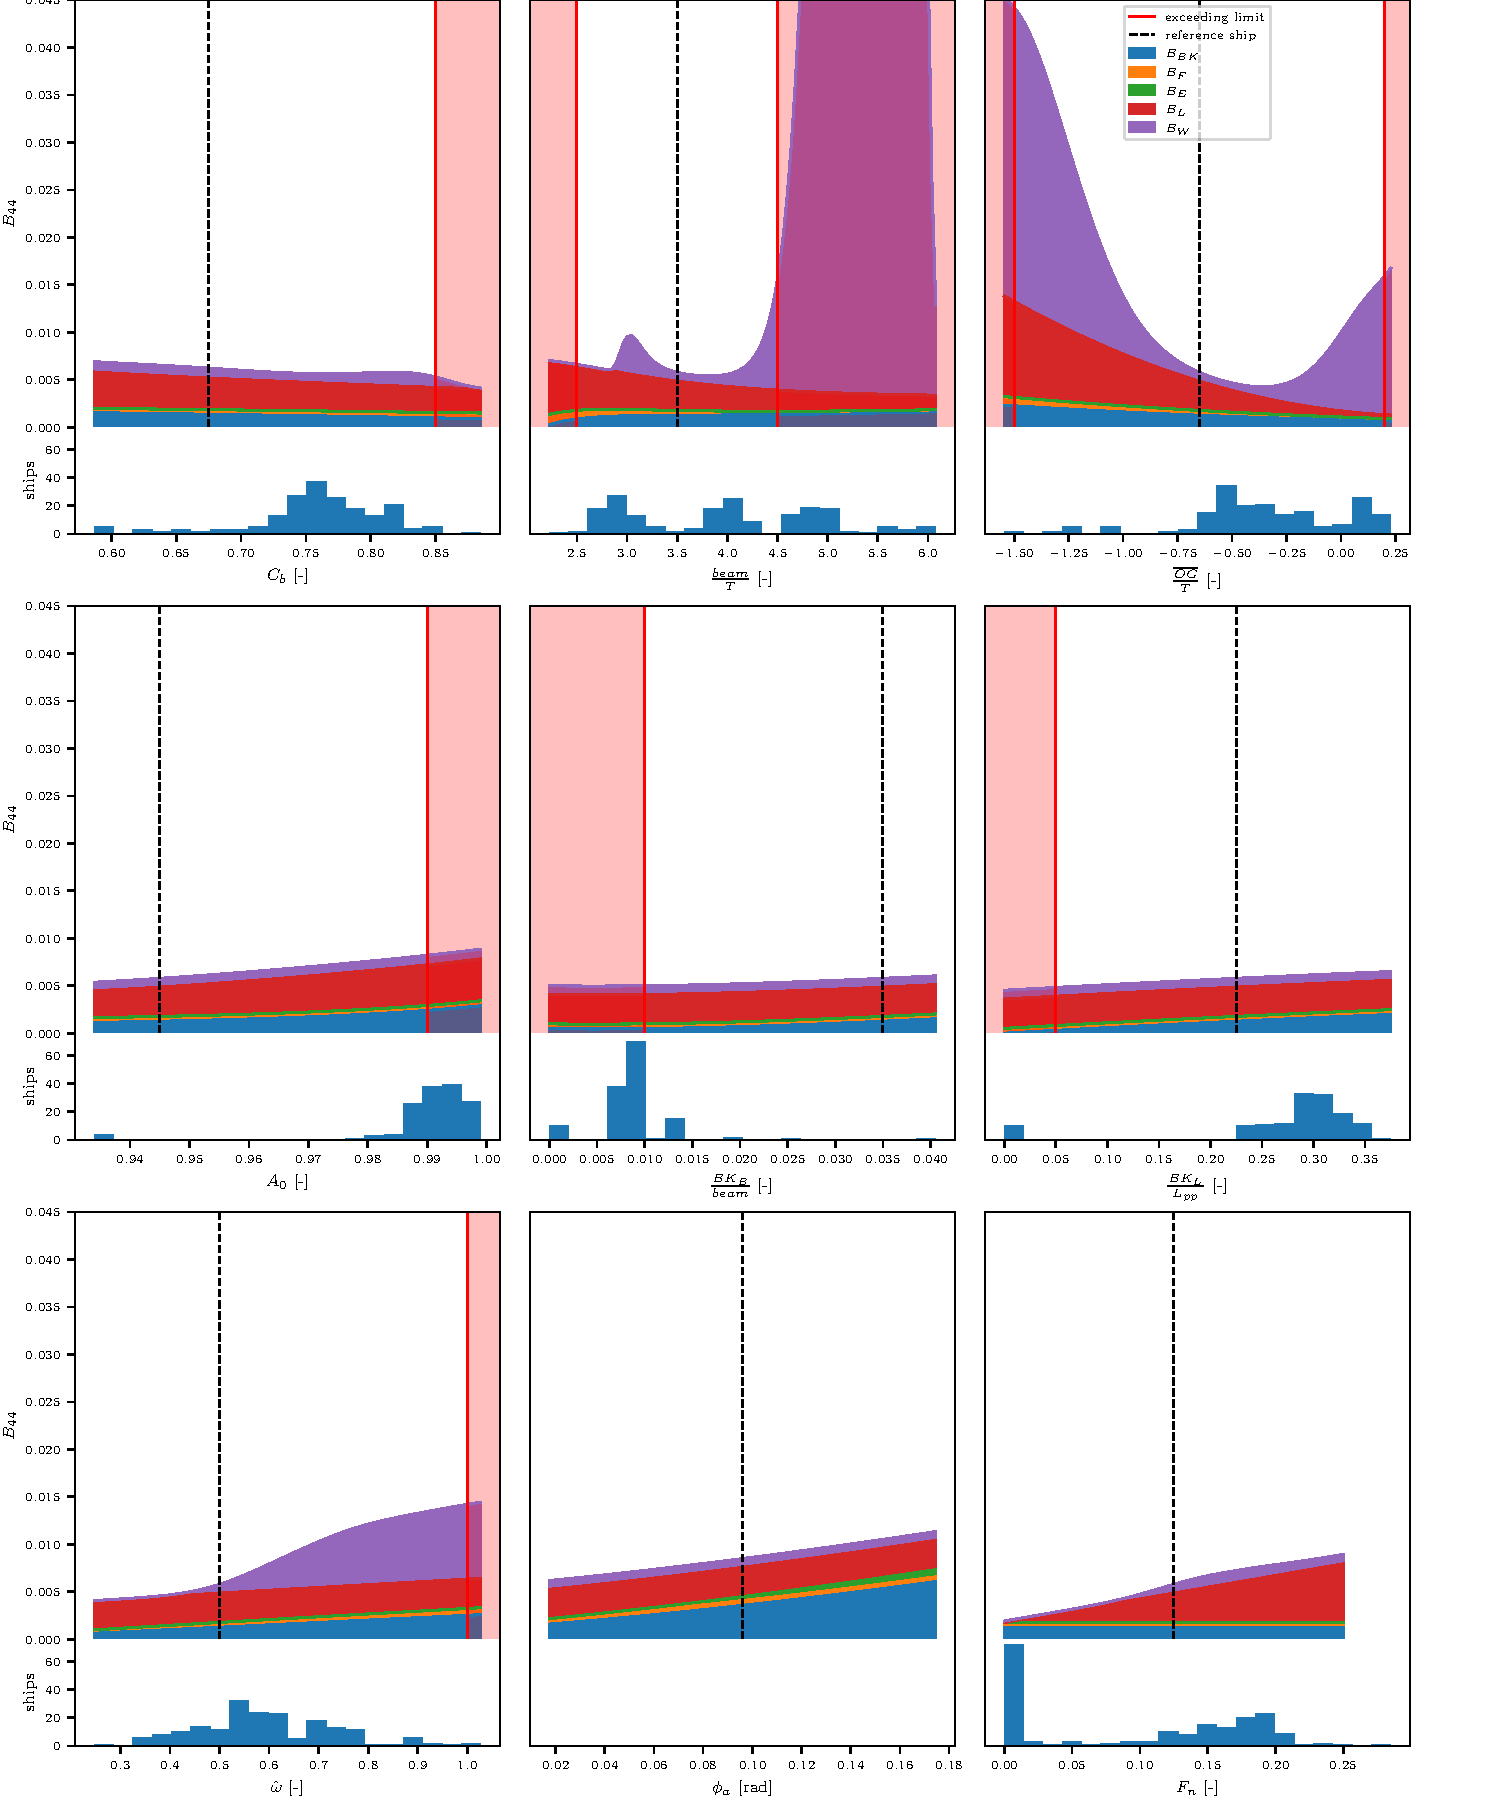
\includegraphics[width=0.8\textwidth]{figures/SI-sensitivity.pdf}
        \vspace{-0.1cm}
    \caption{SI-method input parameter variation and data base ships}
    \label{fig:SI_sensitivity}
\end{figure}
